In this appendix, we will describe the process of fitting and
removing a polynomial from $N$ data points $(x_i, y_i)$ which undergoes a
random walk. The polynomial will be fitted using a least squares minimisation.
The $x_i$ are the independent points at which $y_i$ (which undergoes a random
walk) is measured. We begin by defining the least-squares fitting method then
go on to calculate the residual for several different degrees of polynomial.
This introduces the method in a generic setting which is then applied in
Section~\ref{sec: random walk models part II} to calculate the mismatch for a
GW signal which undergoes a random walk, but in which the search minimises the
mismatch over the search frequency and frequency derivative.

\subsection{Least squares fitting of a polynomial}
Given $N$ data points $x_{i}$, $y_{i}$, we define the residual from a least-squares
polynomial fit of order $k$, as
\begin{equation}
    r_i^{(k)} = y_{i} - y^{\textrm{(k)}}_{i},
\end{equation}
where
\begin{equation}
y^{\textrm{(k)}}_{i} = a_{0} + a_{1}x_{i} + a_{2}x_{i}^{2} + \dots
                                                           + a_{k} x_{i}^{k},
\end{equation}
is a polynomial of degree $k$.

Then the residual which we want to minimise is
\begin{equation}
R^{2} = \s{i=1}{N}\left(r_i^{(k)}\right)^{2}
      = \s{i=1}{N}\left(y_{i} - \left(a_{0} + a_{1}x_{i} + a_{2}x_{i}^{2} +
        \dots + a_{k} x_{i}^{k}\right)\right)^{2}.
\end{equation}
Partial differentiation with respect to the parameters $a_{i}$, yields $k$
simultaneous equations. Writing these as a matrix and then solving
for the best fit, $\hat{y}^(k)_i$, it can be shown \citep{WolframLeastSquares} that
\begin{align}
\hat{y}^{\textrm{(k)}}_{i} & = X \left(X^{T}X\right)^{-1} X^{T} y_{i} & \textrm{where} & &
X & = \left[\begin{array}{ccccc}
1 & x_{1} & x_{1}^{2} & \dots & x_{1}^{k} \\
1 & x_{2} & x_{2}^{2} & \dots & x_{2}^{k} \\
\vdots & \vdots & \vdots & \vdots & \vdots \\
1 & x_{n} & x_{n}^{2} & \dots & x_{n}^{k} \\
\end{array}\right]
\end{align}
Here $X$ is an example of a \emph{Vandermonde} matrix in which the terms follow
a geometric progression. It is useful to note that
\begin{equation}
XX^{T} = \left[\begin{array}{cccc}
N & \s{i=1}{N}x_{i} & \cdots &  \s{i=1}{N}x_{i}^{k} \\
\s{i=1}{N}x_{i} & \s{i=1}{N}x_{i}^{2} & \cdots &  \s{i=1}{N}x_{i}^{k+1} \\
\vdots & \vdots & \ddots & \vdots \\
\s{i=1}{N}x_{i}^{k} & \s{i=1}{N}x_{i}^{k+1} & \cdots &  \s{i=1}{N}x_{i}^{2k}
\end{array}\right].
\end{equation}

Provided that the $x_{i}$ are suitably defined, then an analytic fit can be
found for any $k$, the difficulty lies in inverting the matrix.

\subsection{Least squares fitting a polynomial to a random walk} We now take
the $x_i, y_i$ to be a Gaussian random walk beginning at the origin. To define
this, let $\delta y_{i} \sim N(0, \sigma^{2})$ be independent and identitically
distributed random variables for which their sum generates the random walk:
\begin{equation}
y_{i} = \sum_{j=1}^{i}\delta y_{i}.
\label{eqn: ToyModel RW definition}
\end{equation}
We also set each random walk event to occur according to $x_{i} = i \Delta x$.
Then the residual after fitting and removing a $k^{th}$ order polynomial to the
random walk $y_i$, is
\begin{equation}
r_i^{(k)} = y_{i} - \hat{y}_{i}^{(k)} = y_{i} - X \left(X^{T}X\right)^{-1} X^{T} y_{i}.
\label{eqn: fitted residual}
\end{equation}
This suggests the residual will be similar to the random walk, but modified by
the least squares fitting.  To illustrate this, in Figure~\ref{fig: ToyModelRW}
we plot a simulated random walk along with several fits.
\begin{figure}[htb]
\centering
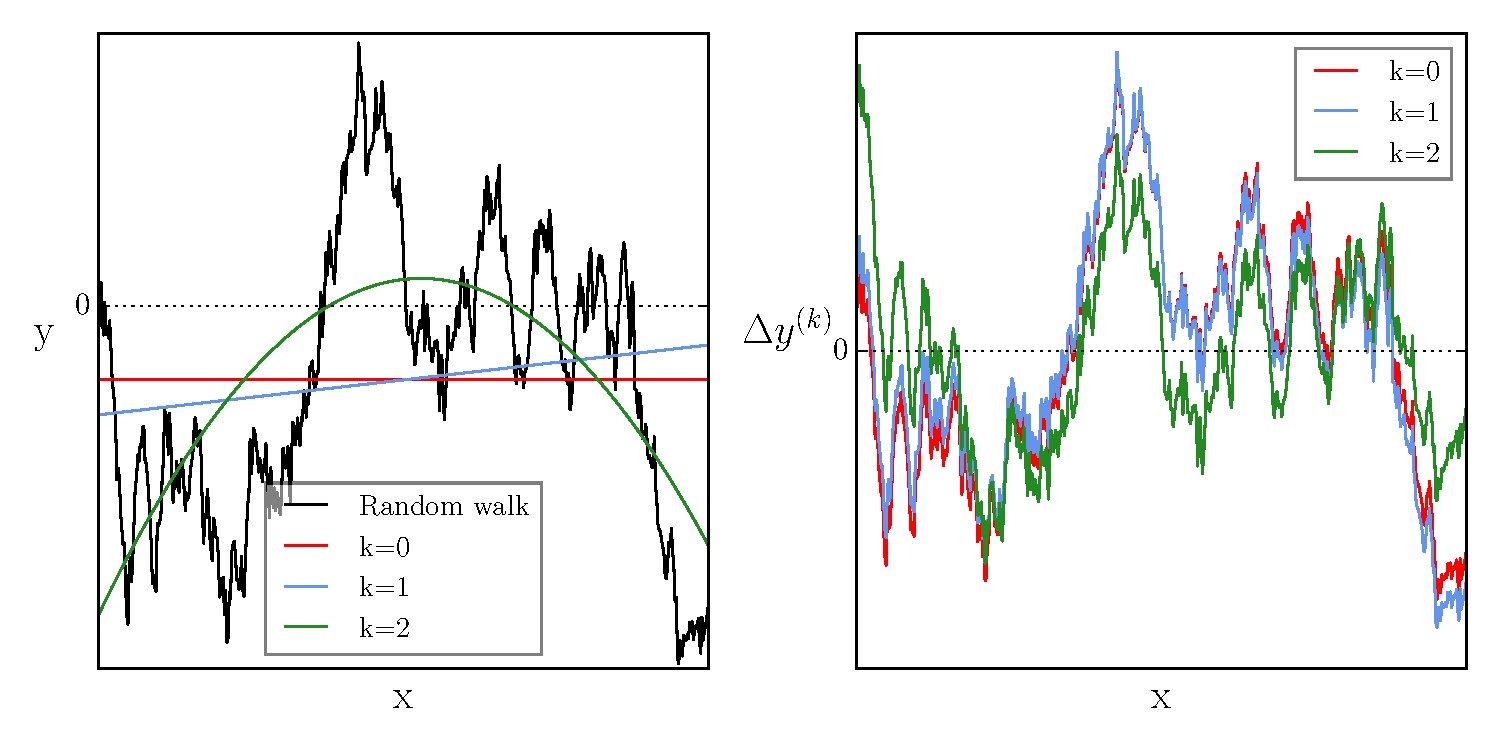
\includegraphics[width=.9\textwidth]{ToyModelRW}
\caption{Example of a random walk on the left along with three polynomial fits
of varying order. On the right is the corresponding residual after subtracting
these fits. A dotted line marks the origin in both plots.}
\label{fig: ToyModelRW}
\end{figure}

\subsection{Zeroth order fitting}

We begin with the case of $k=0$ in which $X^{T} = [1, 1, \dots 1]$ such
that
\begin{equation}
X \left(X^{T}X\right)^{-1} X^{T} = \frac{1}{N} J_{N}
\end{equation}
where $J_{N}$ is the $N\times N$ matrix of ones.  Inserting this into
Eqn.~\eqref{eqn: fitted residual}, the residual from a zeroth order fit is
given by
\begin{equation}
r_i^{(0)}= y_{i} - \frac{1}{N} \s{j=1}{N}y_{j}.
\end{equation}
The zeroth order residual can be interpetted as the removing the
average value $\langle y_i \rangle$ from the random walk: this was illustrated
in Figure~\ref{fig: ToyModelRW}.

%For example the
%expectation after $i$ steps of the original random walk can be shown to be
%zero, therefore the expectation for the zeroth order residual after $i$ steps
%will also be zero.

%This can intuitively be understood from the fact that we started out RW at the origin,
%a zeroth order fit shifts the origin but a random walk should

We can now take expectations to understand the behaviour of the residual when
compared to the original definition of the random
walk in Eqn.~\ref{eqn: ToyModel RW definition}. For example, consider
the mean square translation distance from the origin of a random walk after $i$
steps. For a normal random walk, this has the well known result
\begin{equation}
E[y_{i}^{2}] = i \sigma^{2}.
\label{eqn: RW classic}
\end{equation}
We can calculate the corresponding quantity of the $k=0$ residual by first
noting that
\begin{align}
E\left[y_{i}y_{j}\right] & = E\left[\s{k=1}{i}\delta y_{k} \s{l=1}{j}\delta y_{l} \right] \\
& = \s{k=1}{i}\s{l=1}{j}E\left[\delta y_{k} \delta y_{l}\right] \\
& = \s{k=1}{i}\s{l=1}{j} \delta_{kl} \sigma^{2} \\
& = \sigma^{2}\min(i, j),
\label{eqn: E yiyi}
\end{align}
where $\delta_{kl}$ is the Kronecker delta. Then we have
\begin{align}
\left(r^{(0)}_{i}\right)^{2} & = y_{i}^{2} - \frac{2}{N}\s{k=1}{N}y_{i}y_{k} + N^{-2}\s{k=1}{N}\s{l=1}{N}y_{k}y_{l} \\
& =  y_{i}^{2} - 2 N^{-1} \left(\s{k=1}{i}y_{i}y_{k} + \s{k=i+1}{N}y_{i}y_{k} \right)+ N^{-2}\s{k=1}{N}\left(\s{l=1}{k}y_{k}y_{l} + \s{l=k+1}{N}y_{k}y_{l} \right).
\end{align}
Taking the expectation we have
\begin{align}
E\left[\left(r^{(0)}_{i}\right)^{2} \right] & = \sigma^{2}\left(i - \frac{2}{N}\left(\s{k=1}{i}k + \s{k=i+1}{N}i \right)+ \frac{1}{N^{2}}\s{k=1}{N}\left(\s{l=1}{k}l+ \s{l=k+1}{N}k \right) \right) \\
& = \sigma^{2}\left(\frac{N}{3} - i + \frac{1}{2} + \frac{i^{2}}{N} - \frac{i}{N} + \frac{1}{6 N}\right).
\end{align}
This result can be compared with Eqn.~\eqref{eqn: RW classic}, the expectation
of the squared value for a random walk.  In contrast, the expectation after $i$
steps for the residual random walk depends on the length of data $N$ that was
fitted. It can be shown the expectation has a minimum at $i=N/2$.

To further understand the difference between the random walk and
the residual random walk, let us consider the sum of squares after $N$ steps for
the random walk
\begin{equation}
E\left[\s{i=1}{N} y_{i}^{2}\right] = \s{i=1}{N} i \sigma^{2} =
                               \frac{1}{2}\left(N^{2} + N\right)\sigma^{2}.
\label{eqn: sum of squares}
\end{equation}
On the other hand, the sum of squares for the residual random walk is given by
\begin{equation}
E\left[\s{i=1}{N} \left(r^{(0)}_{i}\right)^{2}\right] = 
\frac{1}{6}\left(N^{2} -1\right)\sigma^{2}.
\label{eqn: sum of squares k0}
\end{equation}
Comparing equations \eqref{eqn: sum of squares} and \eqref{eqn: sum of squares
k0} we note that, for the leading order term, the coefficient is reduced, but
the power remains the same.

%We verify this behaviour with a simple script that produces a random walk of
%length $N$ then fits and subtracts a $0^{th}$ order polynimial; we then
%calculate the sum of the square residual. In Figure~\ref{fig:
%sum_of_squares_res_oth_order} we repeat this operation multiple times then plot
%the average of the sum of squares for the residual while varying $N$, the
%prediction of Eqn.~\eqref{eqn: sum of squares k0} is also plotted showing
%agreement.
%
%\begin{figure}[ht]
%\centering
%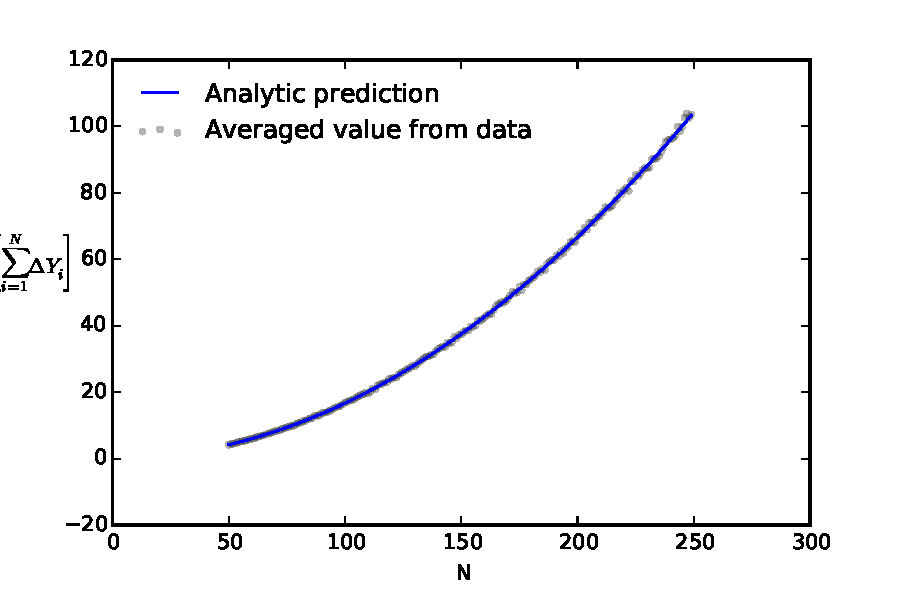
\includegraphics[width=.6\textwidth]{sum_of_squares_res_oth_order}
%\caption{Comparing Eqn.~\eqref{eqn: sum of squares k0} with the averaged sum of squares for a simulated random walk }
%\label{fig: sum_of_squares_res_oth_order}
%\end{figure}

\subsection{First order fitting}
We now consider a first order fitting for which
\begin{align}
\hat{y}^{(1)}_{i} & = X\left(X^{T}X\right)^{-1} X^{T} y_{i} & \textrm{with} &&
X & = \left[\begin{array}{cc}
1 & \Delta x \\
1 & 2 \Delta x  \\
\vdots & \vdots  \\
1 & N \Delta x  \\
\end{array}\right].
\end{align}
Inserting the definitions of $x_{i}$ we can write
\begin{equation}
\left(X^{T}X\right)^{-1} = \frac{1}{N(N-1)}\left[
\begin{array}{cc}
4N+2 & -\frac{6}{\Delta x} \\
 -\frac{6}{\Delta x} & \frac{12}{\Delta x^{2} (N+1)}
\end{array}•
\right] = \Cone.
\end{equation}
For convenience we have defined a symmetric matrix $\Cone$. We then proceed to
define another matrix
\begin{align}
    \mathcal{C}_{ij}^{(1)} & := X\Cone X^{T} \\  & =
\left[\begin{array}{cc}
1 & \Delta x \\
1 & 2\Delta x  \\
\vdots & \vdots  \\
1 & N \Delta x \\
\end{array}\right]
\left[\begin{array}{cc} \Cone_{11} & \Cone_{12} \\ \Cone_{21} & \Cone_{22} \end{array}\right]
\left[\begin{array}{cccc}
1 & 1 & \dots & 1 \\
\Delta x & 2\Delta x & \dots  & N \Delta x
\end{array}\right] \\
& =
\Cone_{11} J_{N} +
\Cone_{12} \Delta x \left[ \begin{array}{cccc}
2 & 3 & \dots & N+1 \\ 3 & 4 & \dots & \vdots \\ \vdots & & & \\  N+1& \dots & \dots & 2N
\end{array}\right] +
\Cone_{22} \Delta x^{2} \left[ \begin{array}{cccc}
1 & 2 & \dots & N \\ 2 & 4 & \dots & \vdots \\ \vdots & & & \\  N& \dots & \dots & N^{2}
\end{array}\right]
\end{align}
We can write $r^{(1)}_{i}$ as a summation by inferring the dependence of the
$i^{th}$ row of each matrix on the $j^{th}$ column
\begin{align}
r^{(1)}_{i} & = y_{i} - \s{j=1}{N}\mathcal{C}_{ij}^{(1)} y_{j}
& \textrm{ where} &&
\mathcal{C}_{ij}^{(1)} & = \Cone_{11} + \Cone_{12}\Delta x (i+j) + \Cone_{22}\Delta x^{2} ij
\end{align}

We have now defined the first order residual. To understand that fitting an
removing a first order polynomial has, we compute the expectation of the
square for the $i^{th}$ term
\begin{align}
\begin{split}
E\left[\left(r^{(1)}_{i}\right)^{2}\right]  =
\frac{1}{15 N \left(N^{2} - 1\right)} &
\left(2 N^{4} - 18 N^{3} i + 9 N^{3} + 78 N^{2} i^{2} - 78 N^{2} i \right.\\
      &\hspace{3mm} + 14 N^{2} - 120 N i^{3} + 180 N i^{2} - 78 N i \\
      &\hspace{3mm} \left. + 9 N + 60 i^{4} - 120 i^{3} + 78 i^{2} - 18 i + 2\right),
\end{split}
\end{align}
which can be compared with the classic result for a random walk given in
Eqn.~\eqref{eqn: RW classic}. Alternatively, comparing with Eqn.~\eqref{eqn:
sum of squares}, the expected sum of squares for the residual random walk is
\begin{equation}
E\left[\s{i=1}{N} \left(r^{(1)}_{i}\right)^{2}\right] 
= \frac{1}{15}\left(N^{2} -4\right)\sigma^{2},
\label{eqn: sum of squares k1}
\end{equation}
as in the zeroth order fit, the power of the leading order term remains the
same, but the coefficient decreases.

\subsection{Second order fitting}
For the residual left after removing a quadratic, the  argument proceeds in much
the same way with
\begin{align}
r^{(2)}_{i} & = y_{i} - \s{j=1}{N}\mathcal{C}_{ij}^{(2)} y_{j},
\end{align}
where
\begin{align}
\mathcal{C}_{ij}^{(2)}  = &\Ctwo_{11} + \Ctwo_{22}\Delta x^{2}ij +
\Ctwo_{33}\Delta x^{4}i^{2}j^{2} \nonumber + \Ctwo_{12}\Delta x(i+j) \nonumber \\
& + \Ctwo_{13}\Delta x (i^{2} + j^2) + \Ctwo_{23}\Delta x^{3}(ij^{2} + i^{2}j),
\label{eqn: MC_2}
\end{align}
and
\begin{equation}
C^{(2)} = \frac{1}{N(N-1)(N-2)}
\left[\begin{matrix}9 N^{2} + 9 N + 6 & - \frac{1}{\Delta{x}} \left(36 N + 18\right) & \frac{30}{\Delta{x}^{2}}\\- \frac{1}{\Delta{x}} \left(36 N + 18\right) & \frac{12 \left(2 N + 1\right) \left(8 N + 11\right)}{\Delta{x}^{2} \left(N + 1\right) \left(N + 2\right)} & - \frac{180}{\Delta{x}^{3} \left(N + 2\right)}\\\frac{30}{\Delta{x}^{2}} & - \frac{180}{\Delta{x}^{3} \left(N + 2\right)} & \frac{180}{\Delta{x}^{4} \left(N + 1\right) \left(N + 2\right)}\end{matrix}\right].
\label{eqn: C_2}
\end{equation}

The expression for the expected square value is too long to write out in full,
but the expected sum of squares for the residual random walk is
\begin{equation}
E\left[\s{i=1}{N} \left(r^{(2)}_{i}\right)^{2}\right] =
 \frac{1}{70}\left(3N^{2} -27\right)\sigma^{2},
\label{eqn: sum of squares k2}
\end{equation}
for which as in the case of the zeroth order and first order residuals, the
power of the leading order term remains unchanged, but the coefficient
decreases.

\subsection{Conclusions}
\label{sec: appendix conclusions}
We now have a method to calculate statistical quantities from the residual
left over after subtracting a $k^{th}$ order polynomial from a random walk.
Considering the sum of squares for a random walk and the residuals in equations
\eqref{eqn: sum of squares}, \eqref{eqn: sum of squares k0},
\eqref{eqn: sum of squares k1}, and \eqref{eqn: sum of squares k2} we find that
the leading order term retains the same
power of $N$ with increasing $k$ but the coefficient of this power gets
smaller. This reflects the improved fitting with the polynomial degrees. We
also note that with each increase in the order of fit we get a limit
on $N$ for which the sum of squares is positive. For zeroth order fitting this
is $N>1$, for first order $N>2$ and for second order $N>3$. This is because in
order to perform a least squares fit, we need at least $k+1$ points to fit.
